\subsection*{2.1}
  % Implement the CE-CC amplifier shown below:
    \begin{figure}[h!]
        \centering
        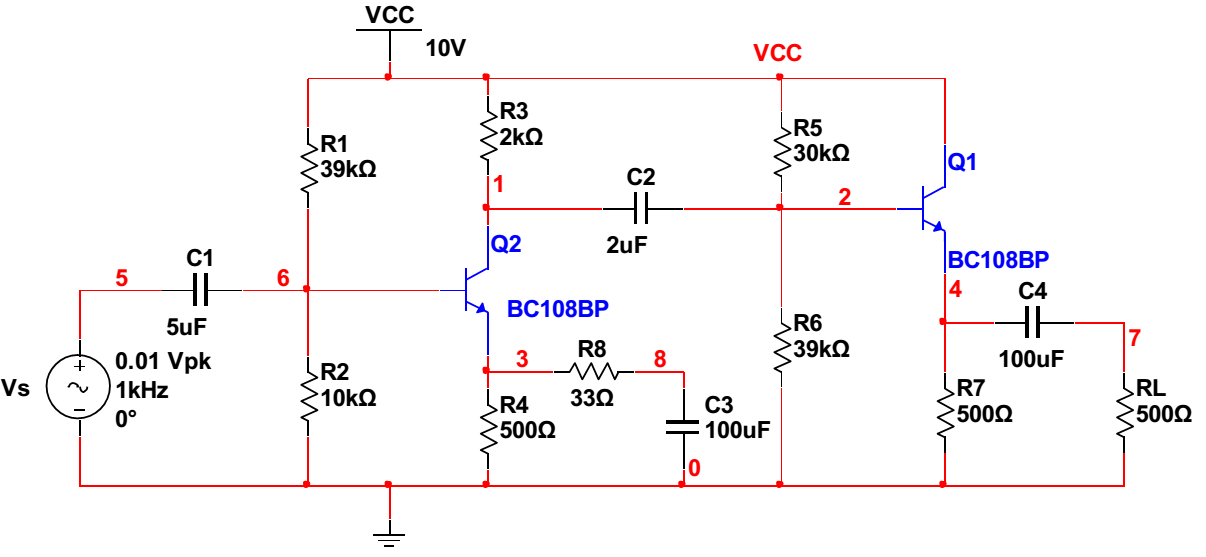
\includegraphics[width=13cm]{fig2-1.png}
        \captionof{figure}{The CE-CC amplifier to be implemented in Task 2.1}
    \end{figure}    

\subsection*{2.2}
  % Using  proper  simulation  techniques,  determine  the  following  parameters  of  the  circuit:
  \subsection*{(i) Midband voltage gain}
  \subsection*{(ii) Input resistance}
  \subsection*{(iii) Output resistance}
  \subsection*{(iv) Lower 3dB frequency}
  \subsection*{(v) Upper 3dB frequency}
  \subsection*{(vi) Output voltage when total harmonics distortion < 5\%}
  2.5471
  
\subsection*{2.3}
  % Summarize  the  circuit  parameters  in  a  table  and  attach  relevant  plots.  Explain  the
  % simulation techniques that you exploited.
  